\section{Objective}
	\subsection{Design a 4-bit R/2R ladder DAC}
		\begin{figure}[H]
			\centering
			\label{obj:1}
			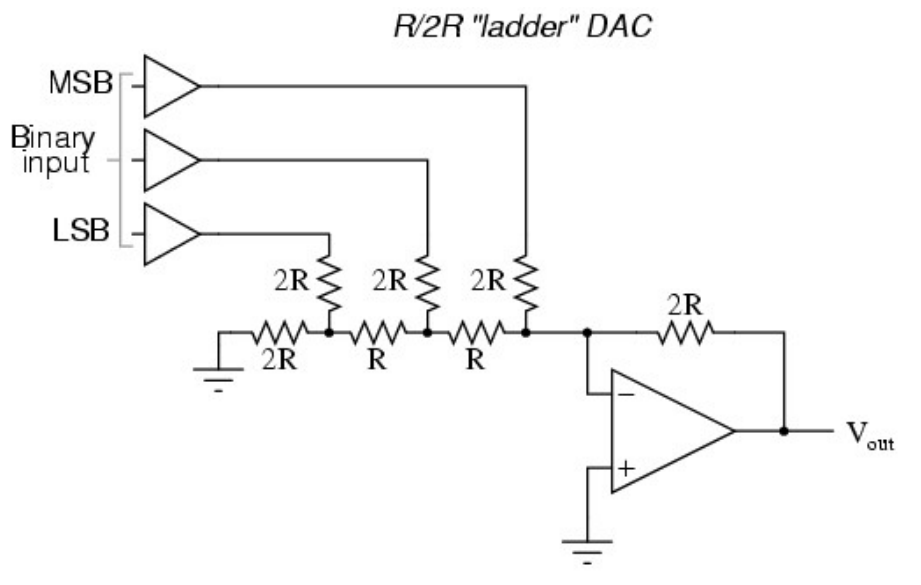
\includegraphics[width=0.6\columnwidth]{images/th1.png}
			\caption{ Circuit diagram for digital to analog conversion }
		\end{figure}
		The DAC circuit consists of a 4-bit R/2R ladder DAC using 741 op amp by choosing components appropriately and testing the circuit. The figure is depicted above. The output voltage of the DAC circuit is given by:
		
		$$V_{out} = \frac{-R_F}{R}\left( \frac{d_1}{2^1} + \frac{d_2}{2^2} + \frac{d_3}{2^3} \right)$$

		where $d_1$ is M.S.B and $d_3$ is L.S.B. In the above circuit, feedback resistance $R_f=2R$. The output impedance of the R-2R network is always R for any number of bits in the network. This Another advantage of the circuit is that it simplifies the design of circuits that use DAC, such as filtering, amplification, etc.

	\subsection{Construct an ADC circuit to convert 2-bit digital input to analog output}
		\hyperref[obj:2]{Figure 3} depicts the conversion's circuit diagram. This circuit employs an $LM339$ comparator and $74147$ priority encoders. The $LM339$ comparator chip compares the analogue input from the DC power source with a reference voltage before passing it to the $74147$ priority encoder circuit. The binary output from the $74147$ chip may then be translated to BCD (Binary coded decimal) format and shown as a decimal digit on a common cathode 7-segment BCD display using the 7447 device. Use three of the four available comparators in $LM339$.
		
		Digital binary output can be produced through $D0$, $D1$, $D2$ and $D3$. It should be noted that the $LM339$ is a quad comparator integrated circuit. Because it has an open collector, it requires pull-up resistors at the comparator's output, as illustrated in \hyperref[obj:2]{Figure 3}. Pull-up resistors of $3k\ohm$ are recommended. When utilising the $LM339$ chip, always connect a $1k\ohm$ resistor in series with the LEDs. The supply voltage to the $LM339$ can be as high as $15V$. Adjust the reference voltage as needed. Before connecting the ADC circuit, learn how the $LM339$ works by connecting one of the comparators and testing the output. $74147$ is a priority encoder with a range of 10 to 4. This IC's input and output are both low. The unused pins should be pulled up to $5V$.
		\begin{figure}[H]
			\centering
			\label{obj:2}
			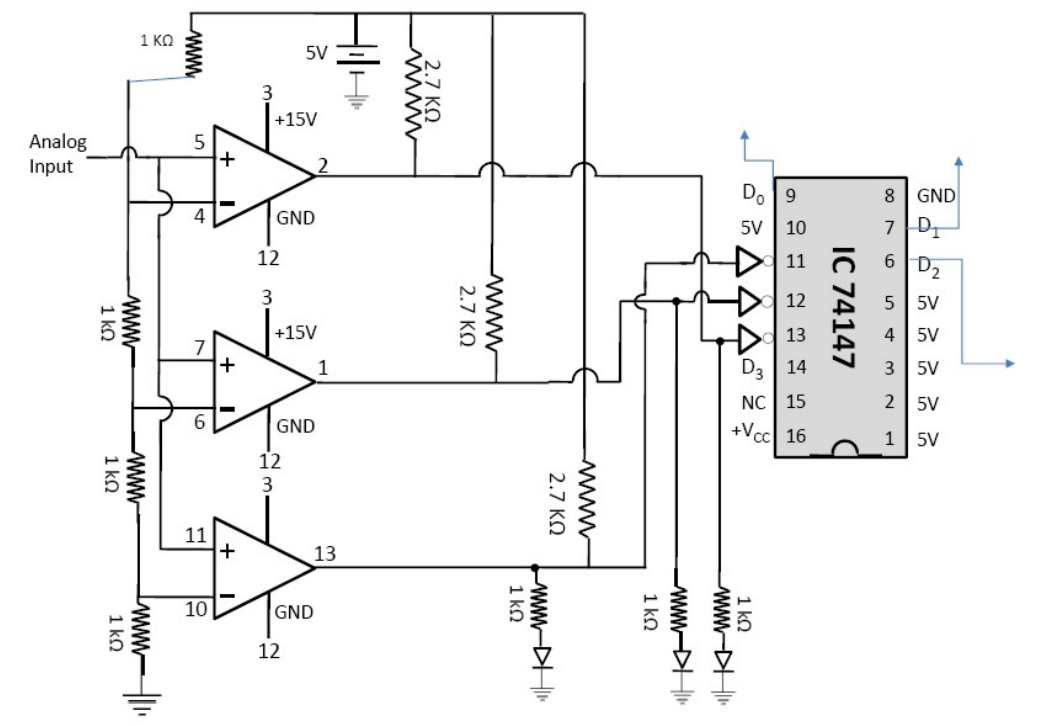
\includegraphics[width=0.8\columnwidth]{images/th2.png}
			\caption{ Circuit diagram for 2-bit binary Analog to Digital conversion }
		\end{figure}

	\subsection{Conversion of the binary display to decimal display}
		After converting analog voltage to binary number, it can be converted to binary coded decimal and displayed on a BCD display. $7447$ is an input active high IC and output active low IC. The output of the $7447$ must be connected to BCD display via a $330\ohm$ resistor.
